A continuación se procede a explicar la construcción del brazo robotico. Para ello, se emplearán los diseños 3D y ciertas imágenes del brazo real en sus etapas de construcción.

La razón de no explicar el proceso integro con imágenes reales del brazo es debido a que no hay suficientes documentos gráficos para ejemplificar el proceso completo y ciertas etapas de la construcción quedarían sin poder ser documentadas.

\begin{figure}[H]
    \centering 
    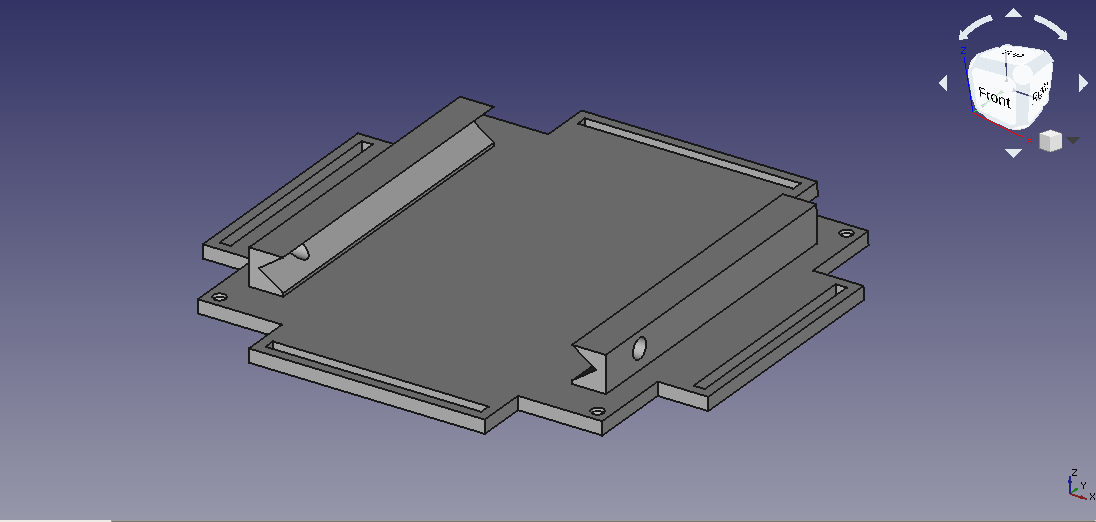
\includegraphics[width=1\linewidth]{pictures/BaseDelBrazoRobotico.png}
    \caption{Base de la caja del brazo robótico}
    \label{fig:base_caja_brazo_robotico}
\end{figure}

\begin{figure}[H]
    \centering 
    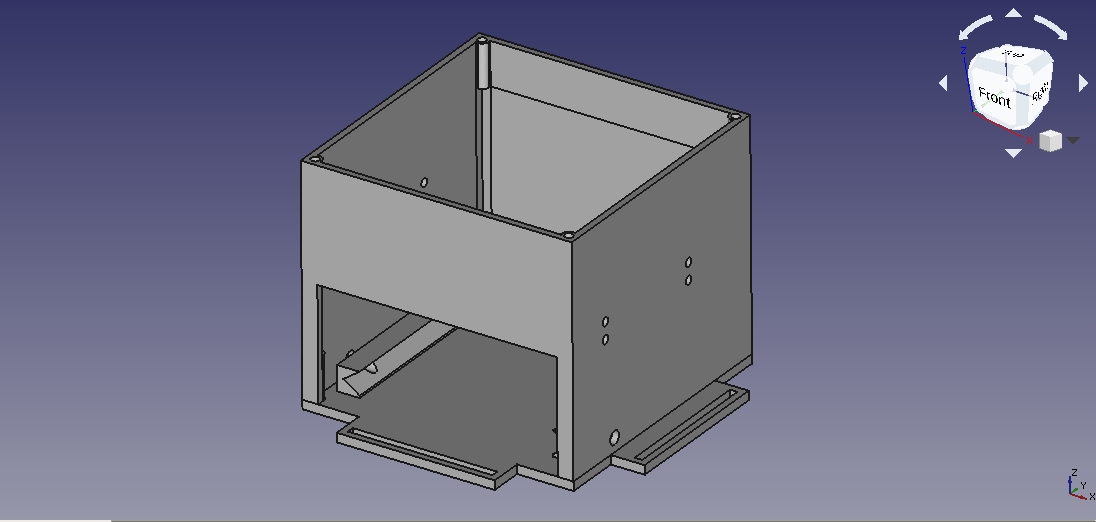
\includegraphics[width=1\linewidth]{pictures/BaseYParedes.png}
    \caption{Base y paredes de la caja del brazo robótico}
    \label{fig:base_paredes_caja_brazo_robotico}
\end{figure}

\begin{figure}[H]
    \centering 
    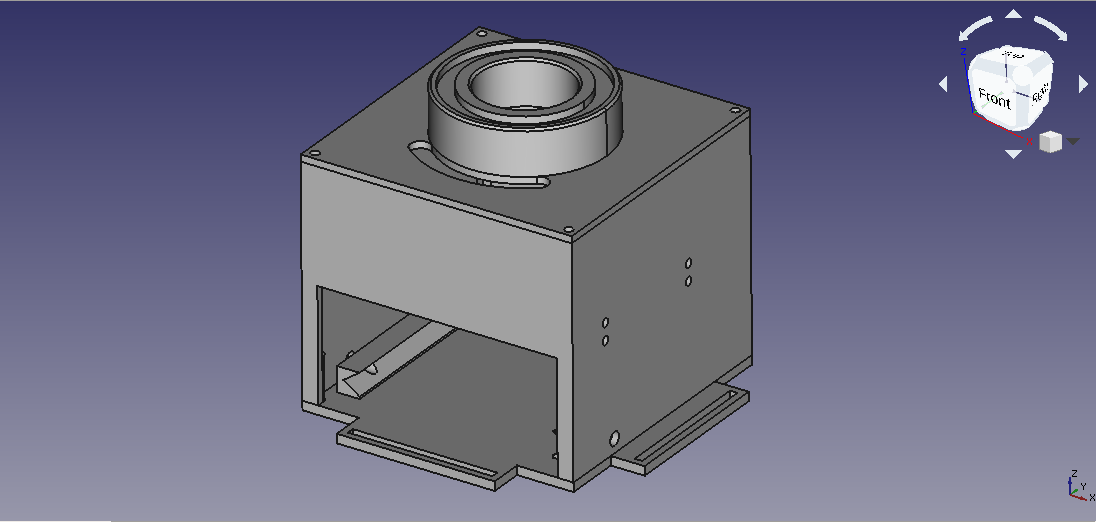
\includegraphics[width=1\linewidth]{pictures/CajaCompleta.png}
    \caption{Caja completa del brazo robótico}
    \label{fig:caja_completa_brazo_robotico}
\end{figure}

Como observamos en las figuras \ref{fig:base_caja_brazo_robotico}, \ref{fig:base_paredes_caja_brazo_robotico} y \ref{fig:caja_completa_brazo_robotico} la caja esta compuesta por 3 piezas y estas se ensamblan verticalmente una encima de otra mediante tornillo de 4x15 cm.
Cabe destacar que esta parte de la estructura es inmóvil y sirve como soporte para la parte móvil.

\begin{figure}[H]
    \centering 
    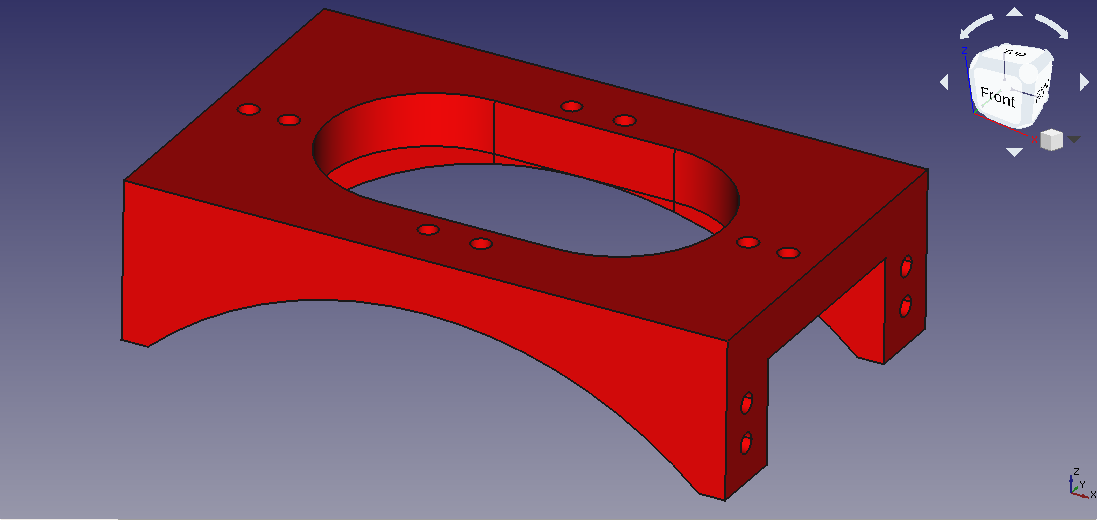
\includegraphics[width=1\linewidth]{pictures/MotorHold.png}
    \caption{Sujeción del motor de la base}
    \label{fig:sujección_motor_base}
\end{figure}

\begin{figure}[H]
    \centering 
    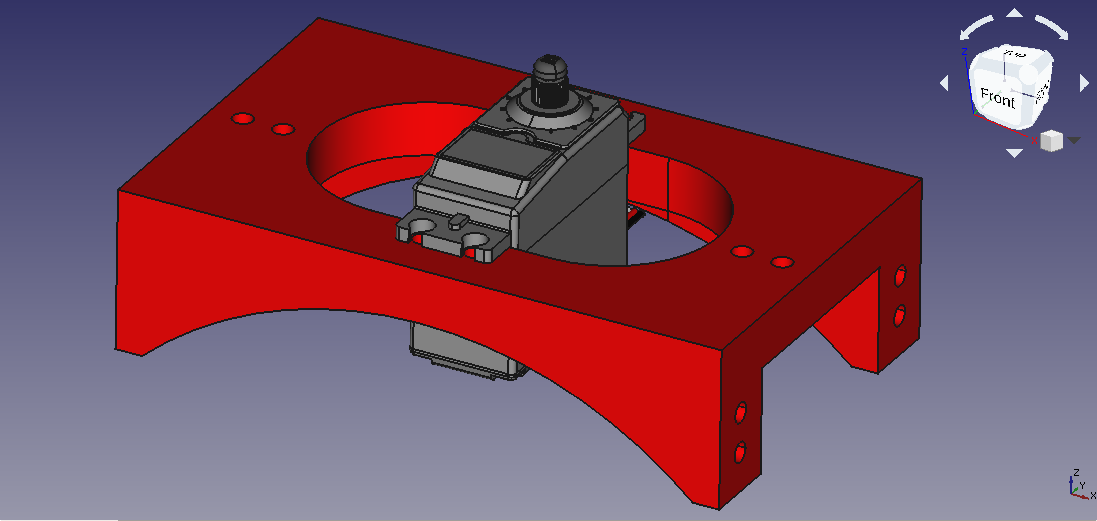
\includegraphics[width=1\linewidth]{pictures/MotorHoldYMotor.png}
    \caption{Motor de la base ensamblado en su soporte}
    \label{fig:motor_ensamblado_soporte}
\end{figure}

\begin{figure}[H]
    \centering 
    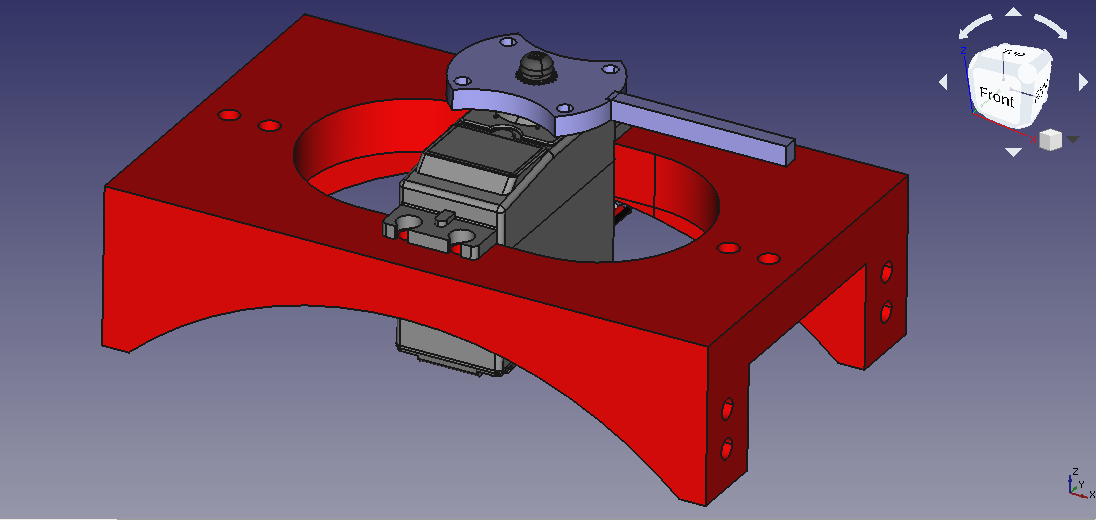
\includegraphics[width=1\linewidth]{pictures/MotorMasPrimeraPieza.png}
    \caption{Primera pieza del sistema de transmisión del movimiento}
    \label{fig:primera_pieza_sistema_transmision}
\end{figure}

\begin{figure}[H]
    \centering 
    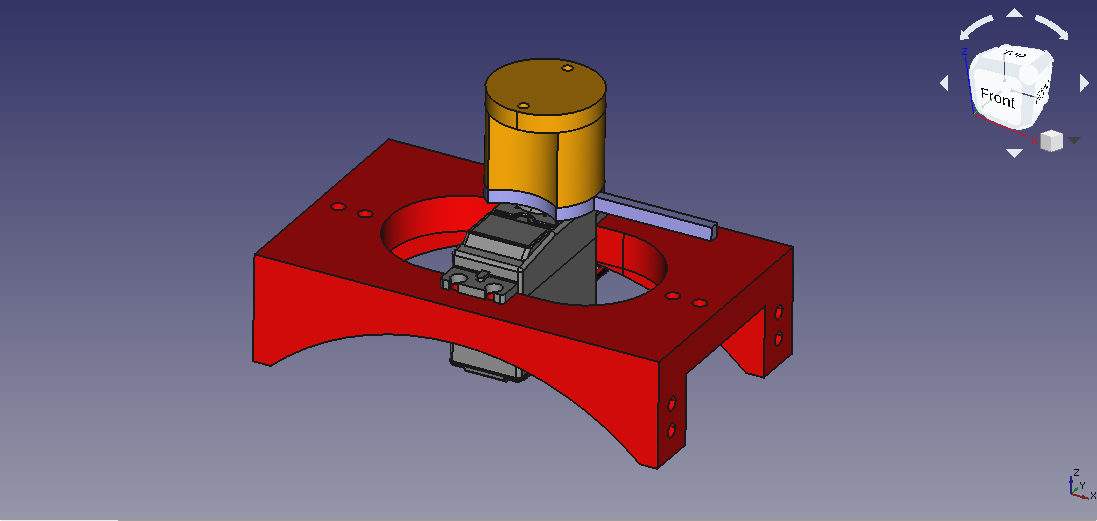
\includegraphics[width=1\linewidth]{pictures/MotorMasSegundaPieza.png}
    \caption{Segunda pieza del sistema de transmisión del movimiento}
    \label{fig:segunda_pieza_sistema_transmision}
\end{figure}

\begin{figure}[H]
    \centering 
    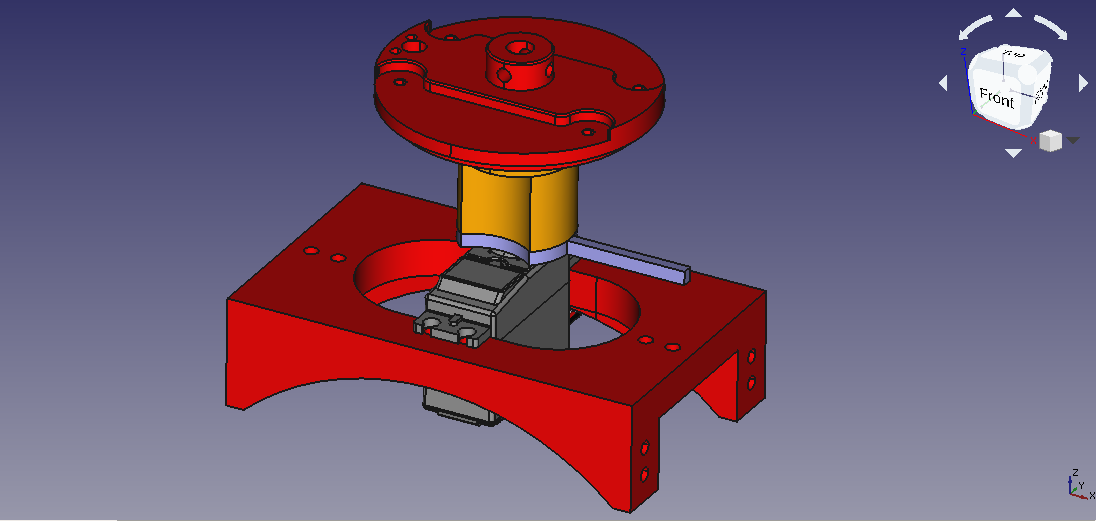
\includegraphics[width=1\linewidth]{pictures/MotorMasTerceraPieza.png}
    \caption{Tercera pieza del sistema de transmisión del movimiento}
    \label{fig:tercera_pieza_sistema_transmision}
\end{figure}

En las figuras \ref{fig:sujección_motor_base}, \ref{fig:motor_ensamblado_soporte}, \ref{fig:primera_pieza_sistema_transmision},
\ref{fig:segunda_pieza_sistema_transmision} y
\ref{fig:tercer_pieza_sistema_transmision} se observan los componentes que servirán para transmitir el movimiento desde el motor a la base giratoria donde ira ensamblado el brazo robótico. Para asegurar el soporte a las paredes y posteriormente el motor al soporte se han empleado tornillos de 4x15 mm. Para los componentes que servirán para transmitir el movimiento, se han empleado tornillos de 3x10 mm debido a que las piezas son mas pequeñas y es necesario que los tornillos ocupen menos espacio.

\begin{figure}[H]
    \centering 
    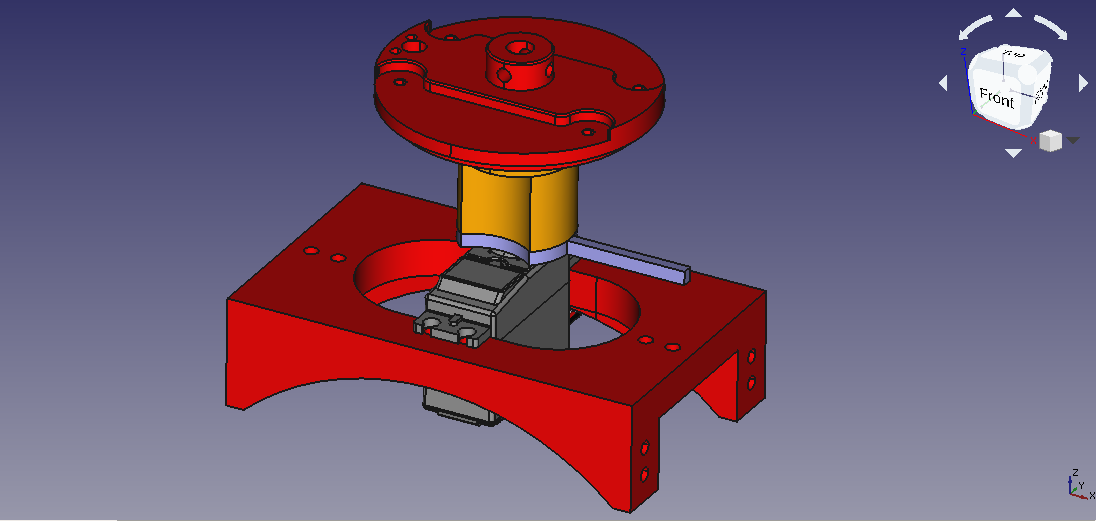
\includegraphics[width=1\linewidth]{pictures/MotorMasTerceraPieza.png}
    \caption{Tercera pieza del sistema de transmisión del movimiento}
    \label{fig:tercera_pieza_sistema_transmision}
\end{figure}